
\subsection{Model Setup}
\subsubsection{Model Domain}
The domain of the model is bounded by longitudes $\phi_E=-180^{\circ}$ and $\phi_W=-180^{\circ}$ and latitudes $\theta_N=80^{\circ}$ and $\theta_S=-80^{\circ}$ with periodic boundary conditions in the zonal direction.
 The depth profile has 15 layers with grid stretching (\cref{fig:gridstrech}). The grid stretching relation is such that surface layers are much shallower than deep water layers. There are $90 \times 40$ horizontal grid points to make a $4^{\circ} \times 4^{\circ}$ resolution model.
 
 \begin{figure}[H]
 	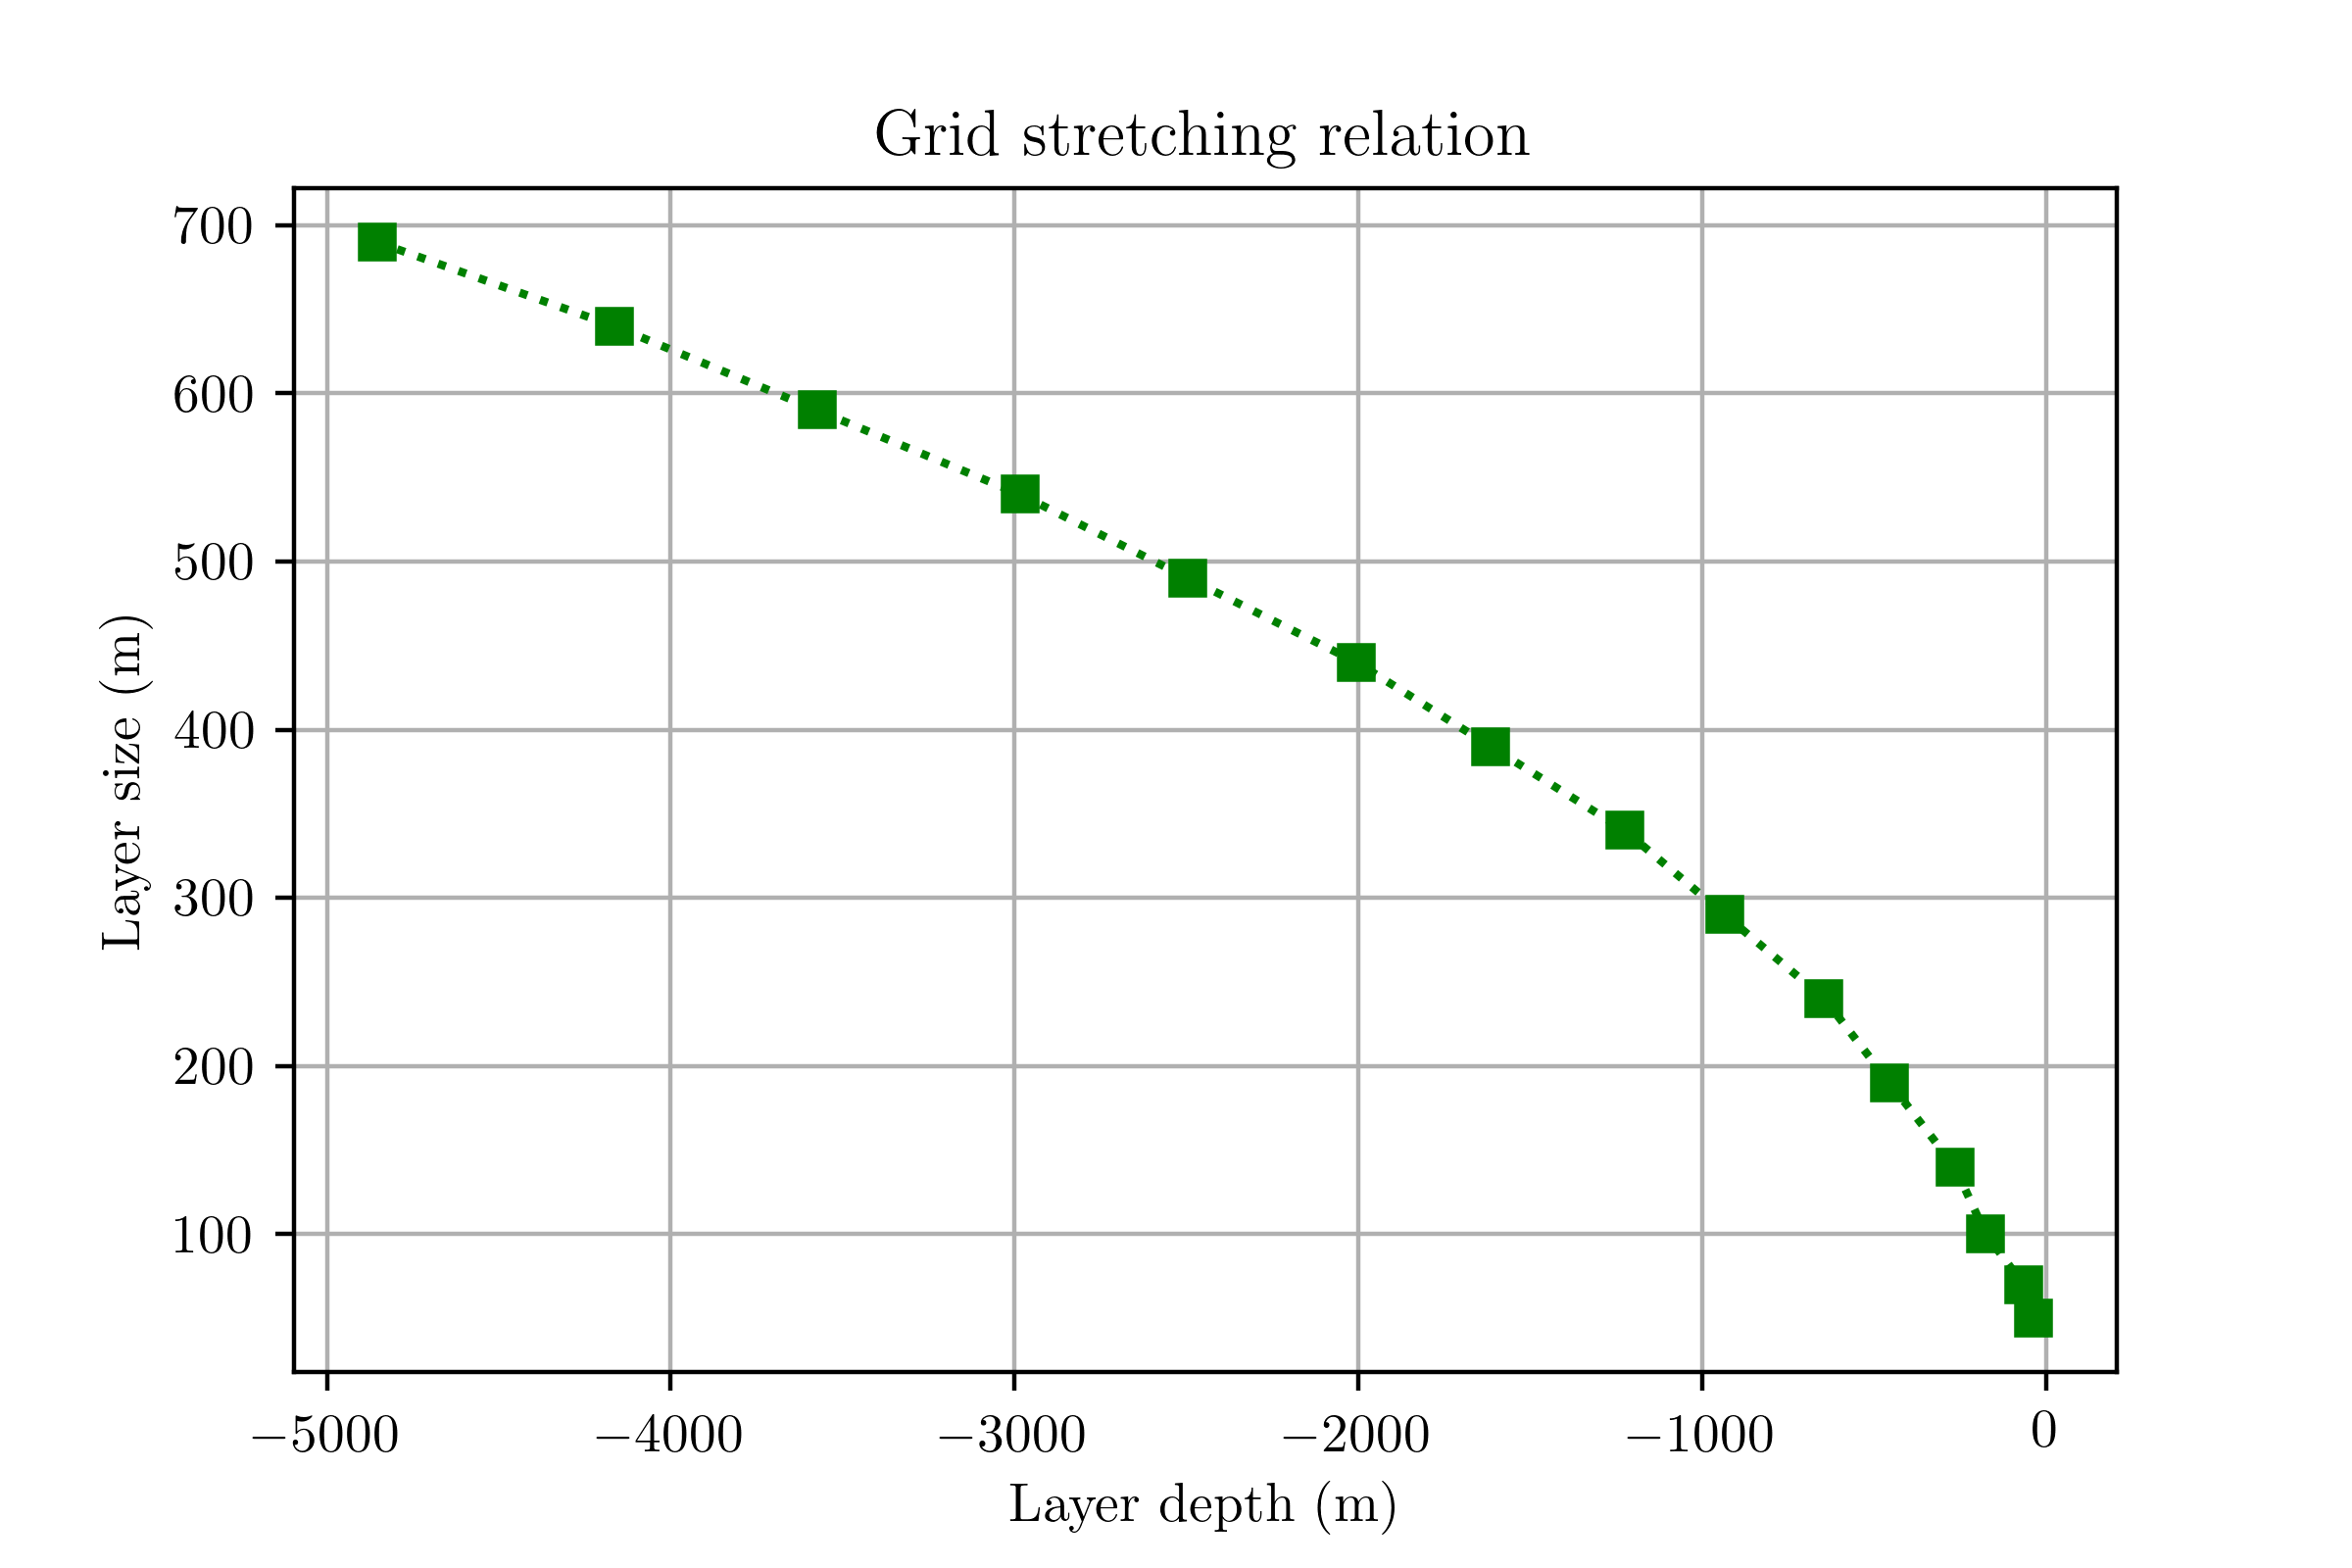
\includegraphics[width=\linewidth]{grid_stretching.png}
 	\caption{Grid stretching relation used for the model setup. Showing the size of the layer for each layer. Upper layers are shallower than deep water layers.}
 	\label{fig:gridstrech}
 \end{figure}

\subsubsection{Surface Forcings}\label{sec:forcing_ideal}
The Veros setup used in this paper has restoring boundary conditions. These restore the boundary at the surface of the oceanic basin to a forcing field for Sea Surface Temperature (SST), Sea Surface Salinity (SSS), wind stress ($\tau$) and heat flux.
Choosing the correct forcing for the ocean is important. It is known that in general circulation models the MOC is sensitive to small changes in surface forcings (\cite{Milliff1999May}). Attempts at making these forcings highly idealized have often been made in the past with varying rates of success(\cite{bryan1987parameter}; \cite{Mulder2017Jul}). We note the fact that using idealized forcings will induce errors, especially in the shape of the thermohaline circulations. The use of idealized forcings is however justified here, because we are only interested in large scale features of the meridional overturning and wind-driven circulations.

Several methods were explored when making these idealized forcings. In the \cite{Mulder2017Jul} paper an analytic forcing profile was used for wind stress, SST, and SSS (\cref{fig:idealized_forc}). However, Veros is a seasonally forced model, using simplified forcings would thus fail to capture seasonal changes in the SST. There have been studies suggesting that these seasonal forcings can have large effects on the strength of the meridional overturning circulation (\cite{schmittner2001seasonally}). Here we propose to take the SSS and SST profiles as zonal means of realistic forcings. We use $1^{\circ} \times 1^{\circ}$ forcings from the European Centre for Medium-Range Weather Forecasts (ECMWF) public dataset as a basis (\cite{ECMWFForc}). While the zonal wind stress is set to the simple profile proposed by \cite{bryan1987parameter}. The choice of this analytic profile was made over a zonally averaged forcing mirrored along the equator ($\mu(\tau_x)$). These forcings proved to be problematic in the polar regions (\cref{fig:tau_profile}). Both forcings were initially tested on the present-day configuration to see which most accurately captures the present-day MOC. After some initial tests, we found that $\mu(\tau_x)$ is very weak in the sub polar regions and subsequently fails to force the North Atlantic Deep Water formations (NADW).
\end{multicols}
%example full width overturning

\begin{figure}[H]
\begin{subfigure}{.5\textwidth}
	\caption{net monthly surface heat flux ($Wm^{-2}$)}
	\label{fig:qnet}
	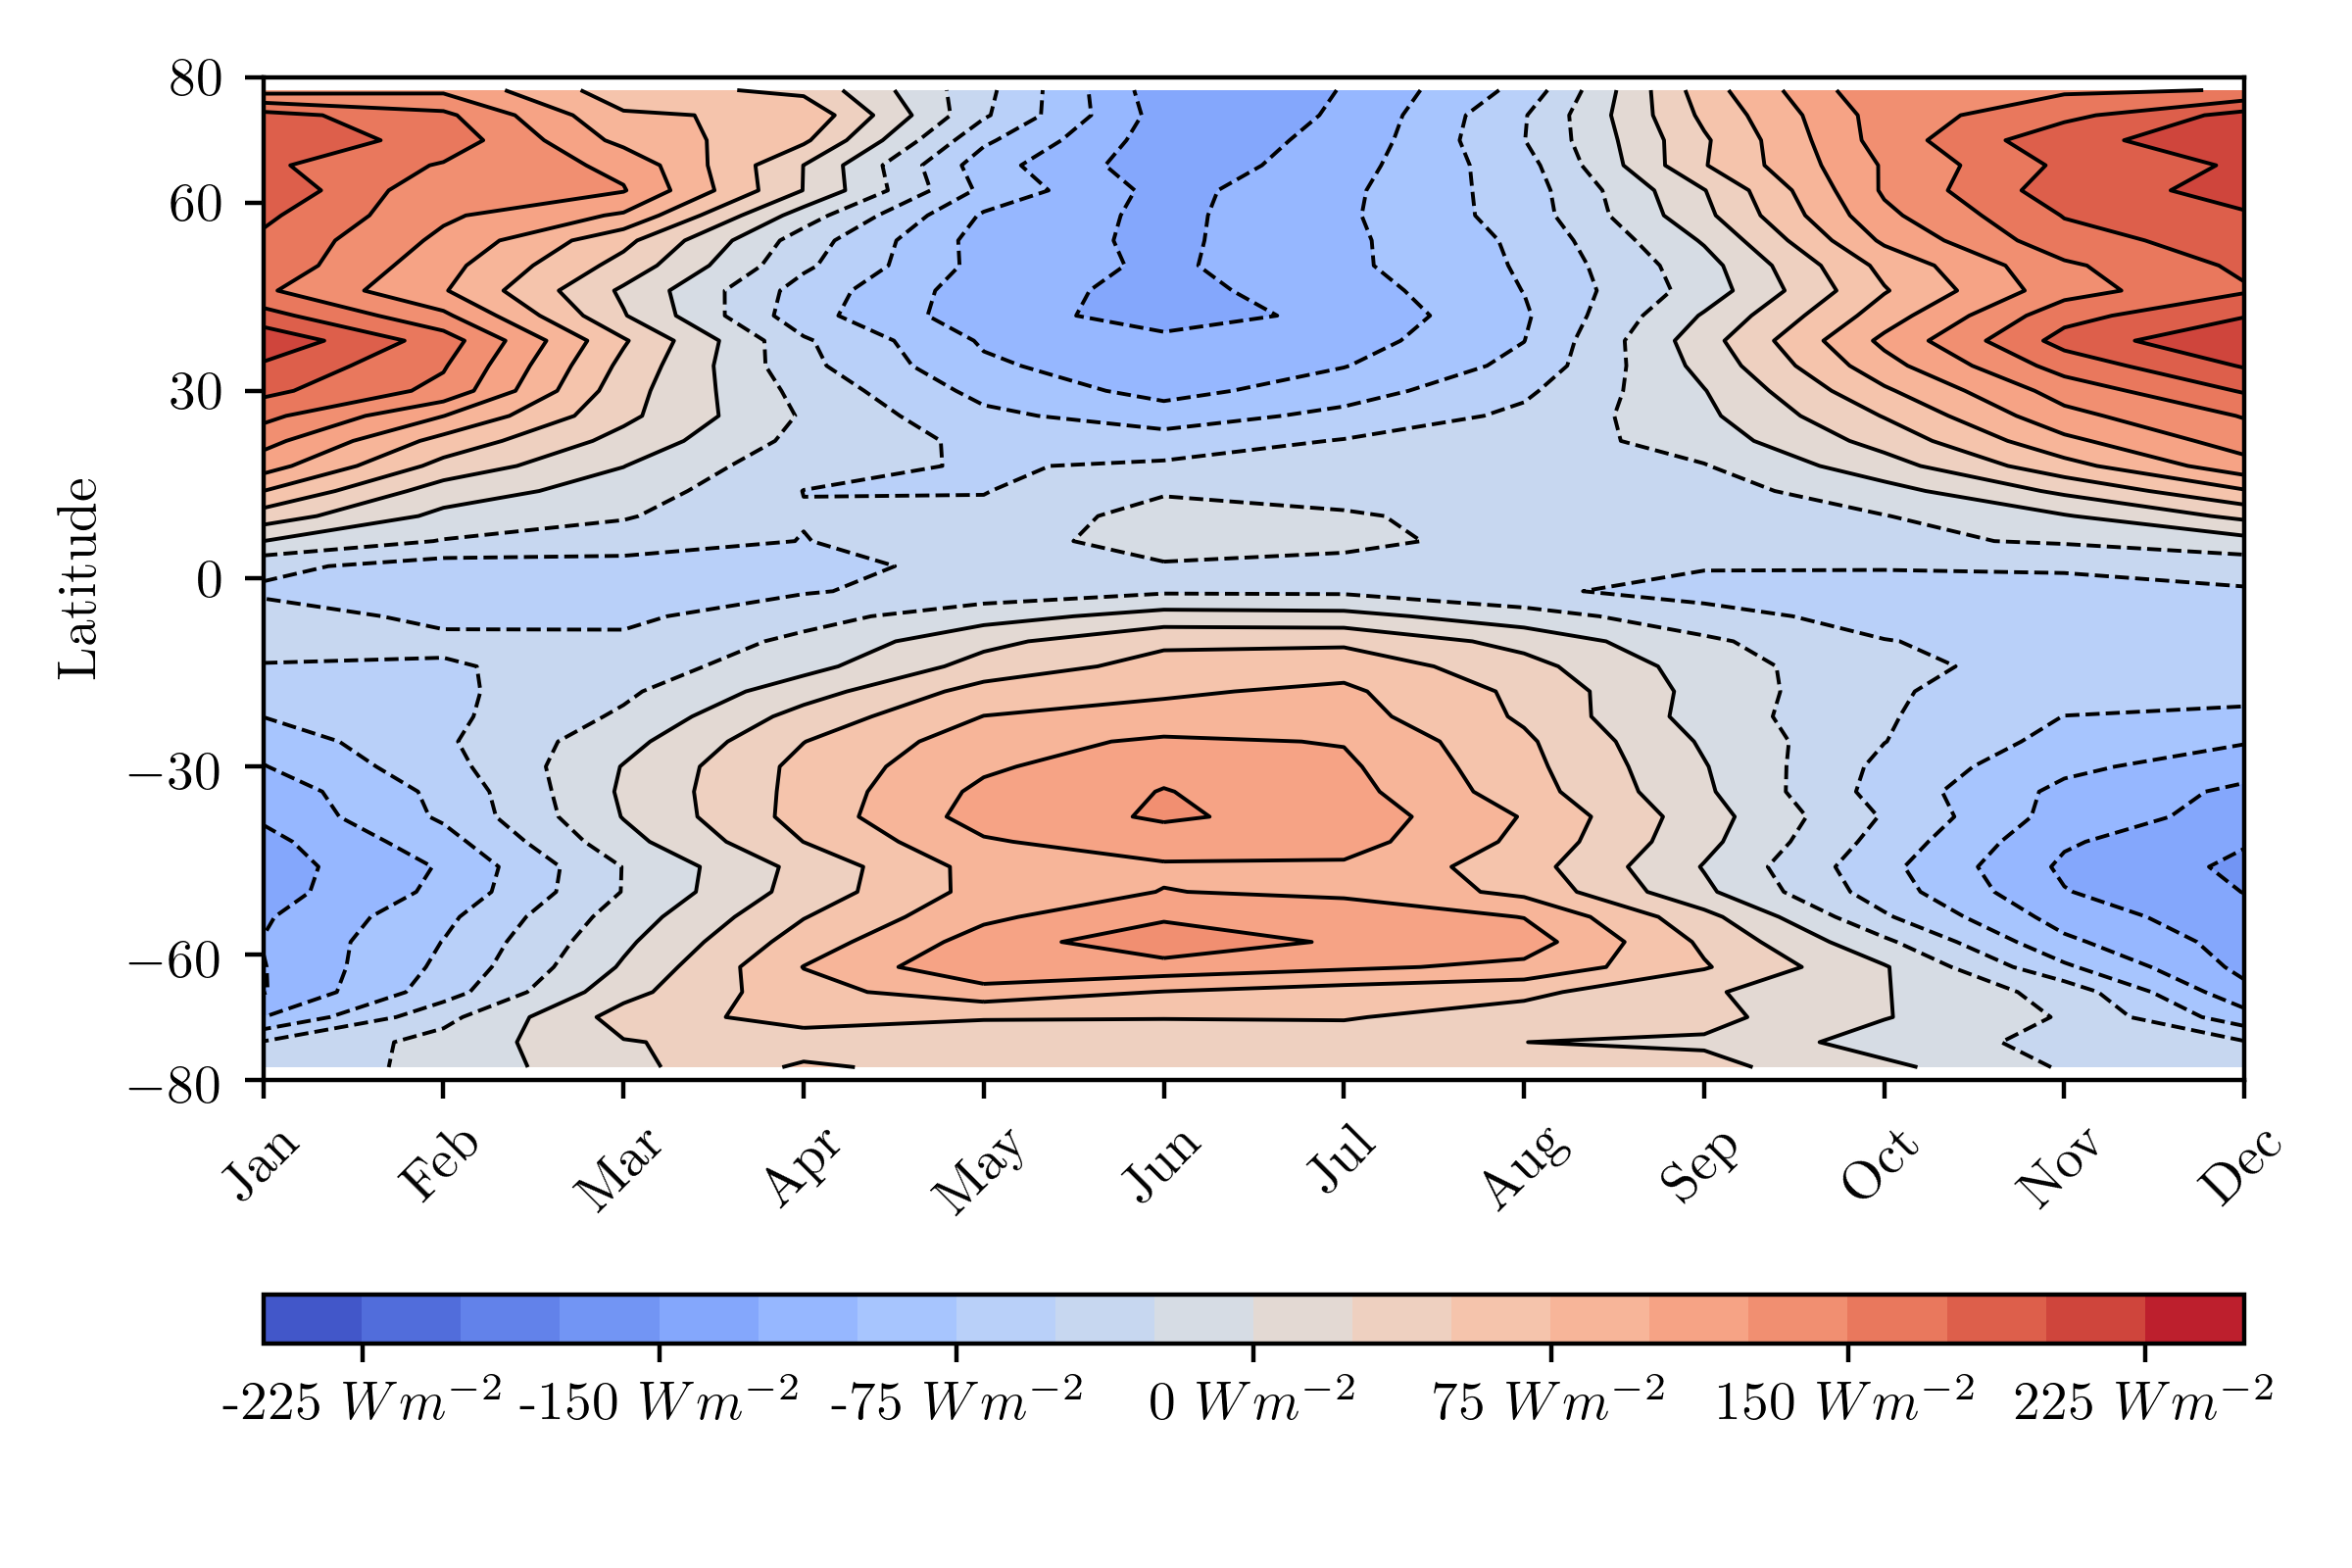
\includegraphics[width=\linewidth]{q_net_profile.png}
\end{subfigure}
\begin{subfigure}{.5\textwidth}
	\caption{SST profile ($^{\circ}C$)}
	\label{fig:sst_profile}
	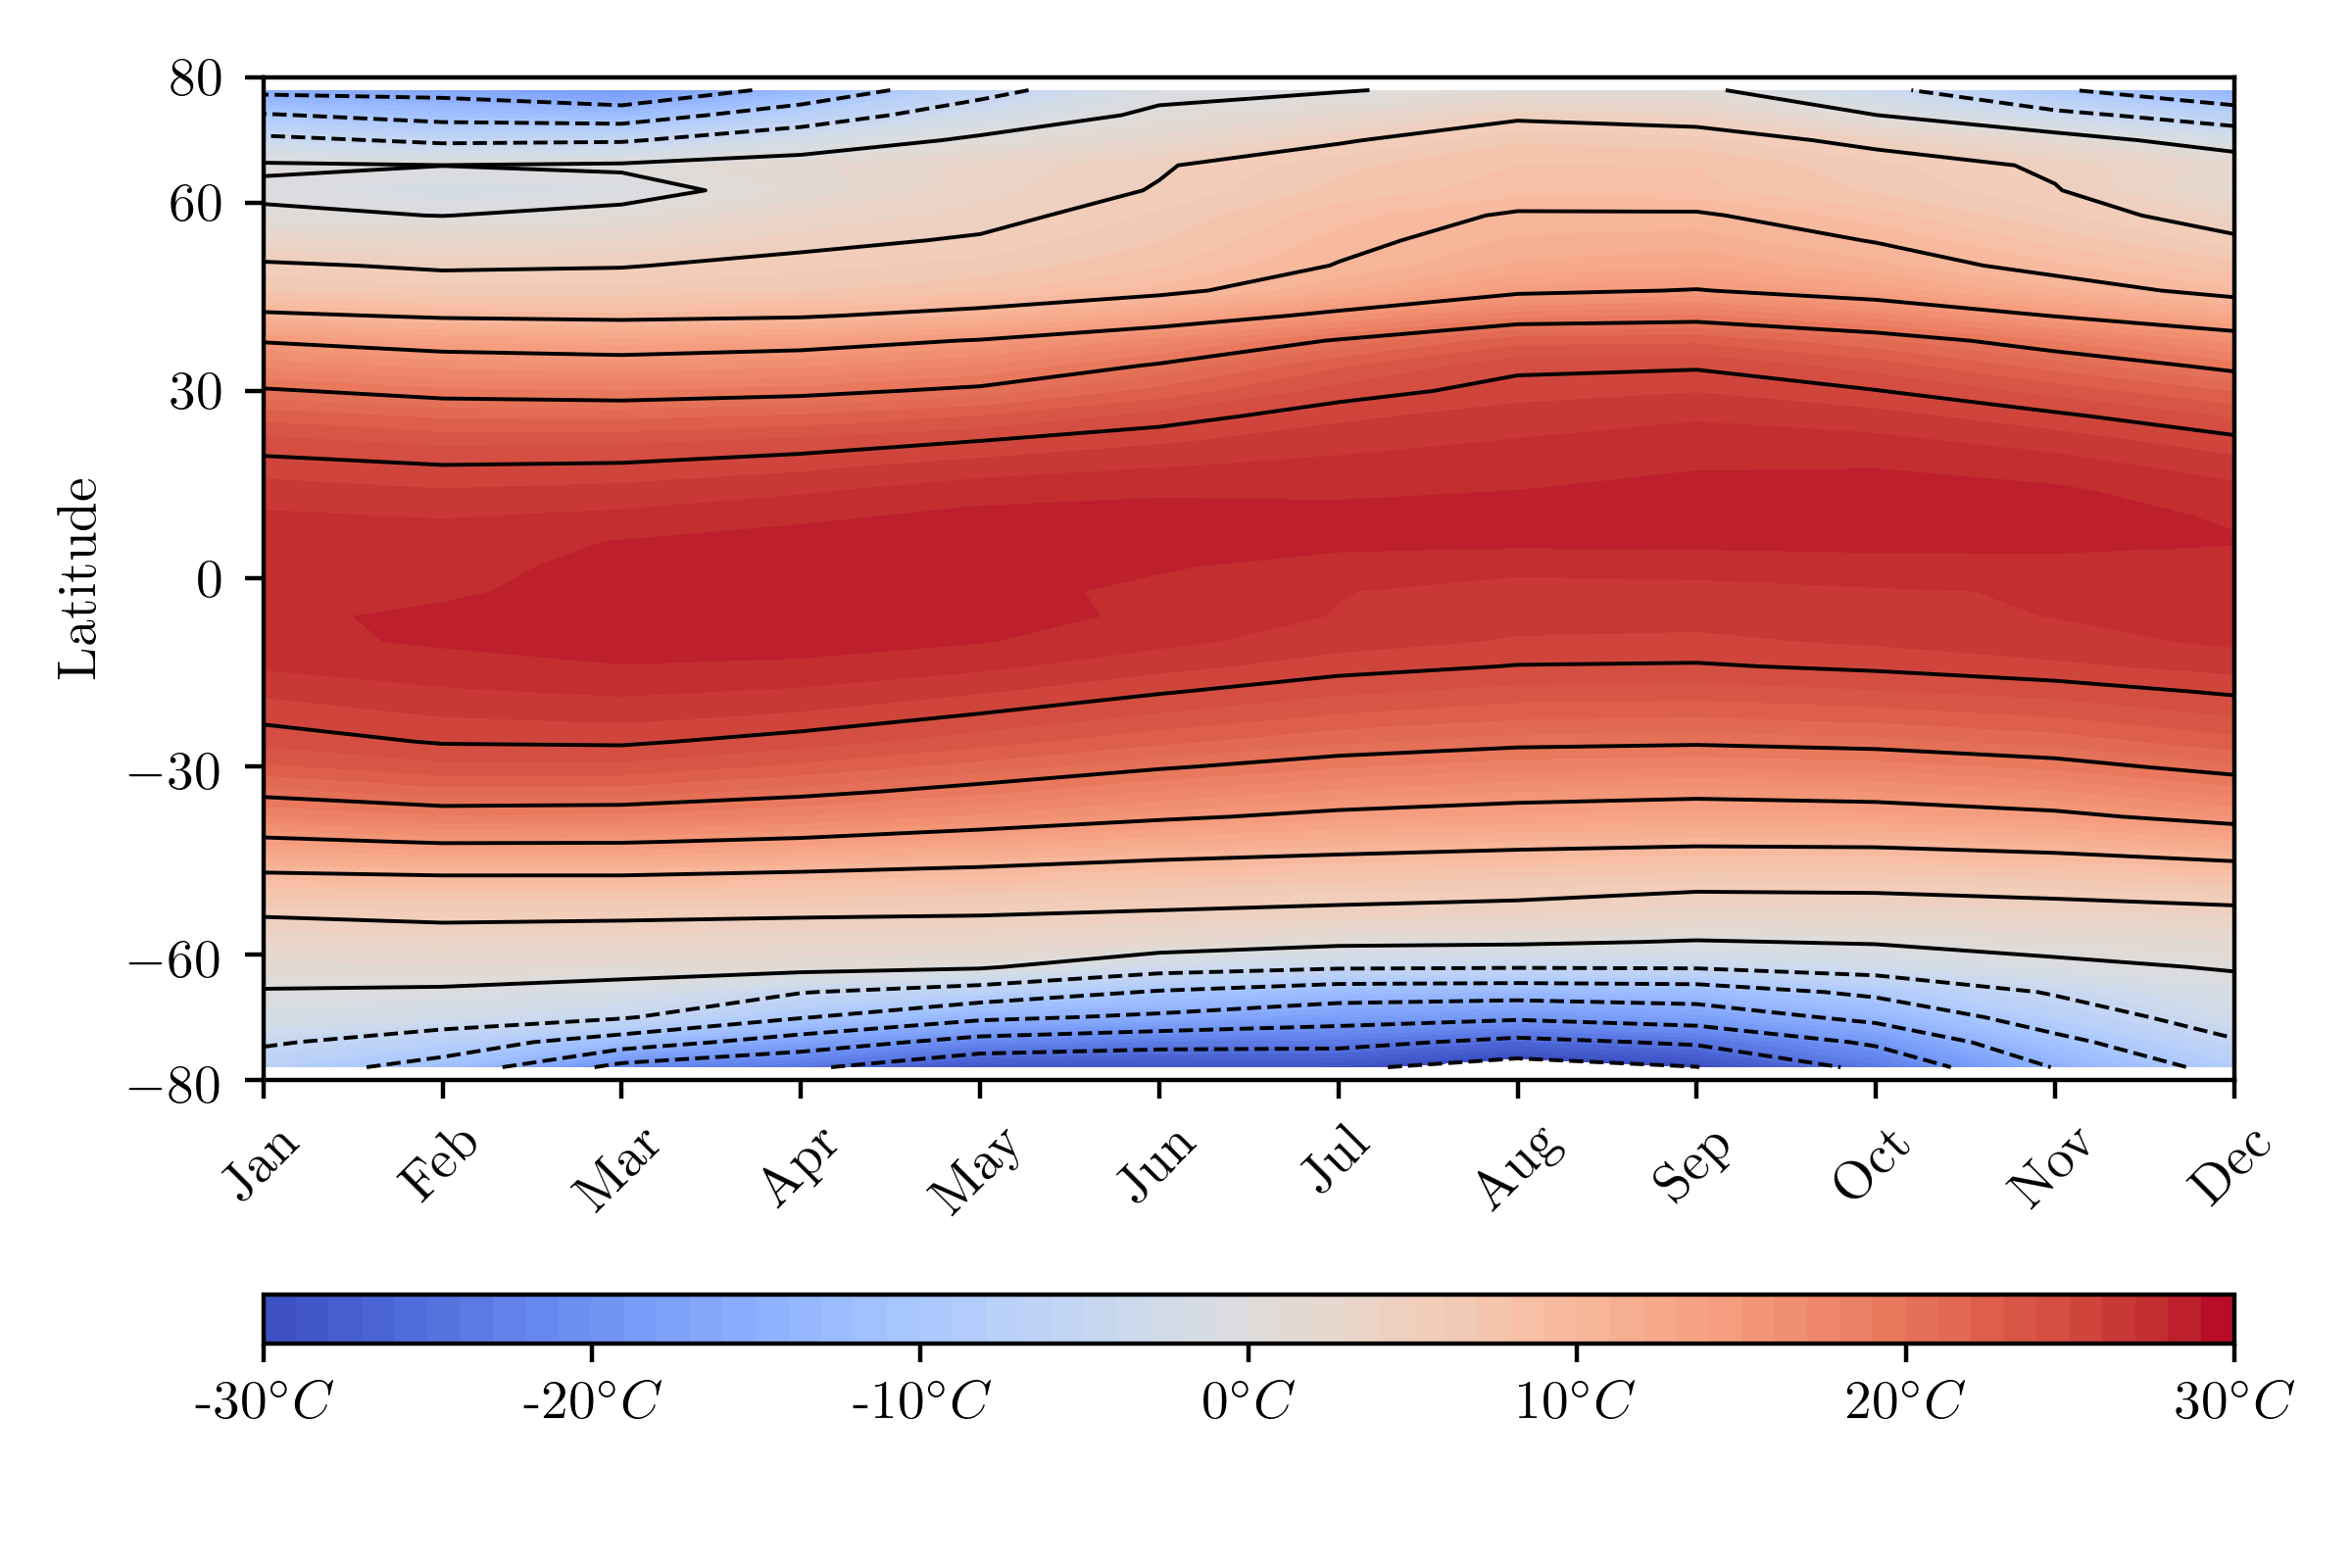
\includegraphics[width=\linewidth]{sst_profile.png}
	
\end{subfigure}
\begin{subfigure}{.5\textwidth}
	\caption{SSS profile ($psu$)}
	\label{fig:sss_profile}
	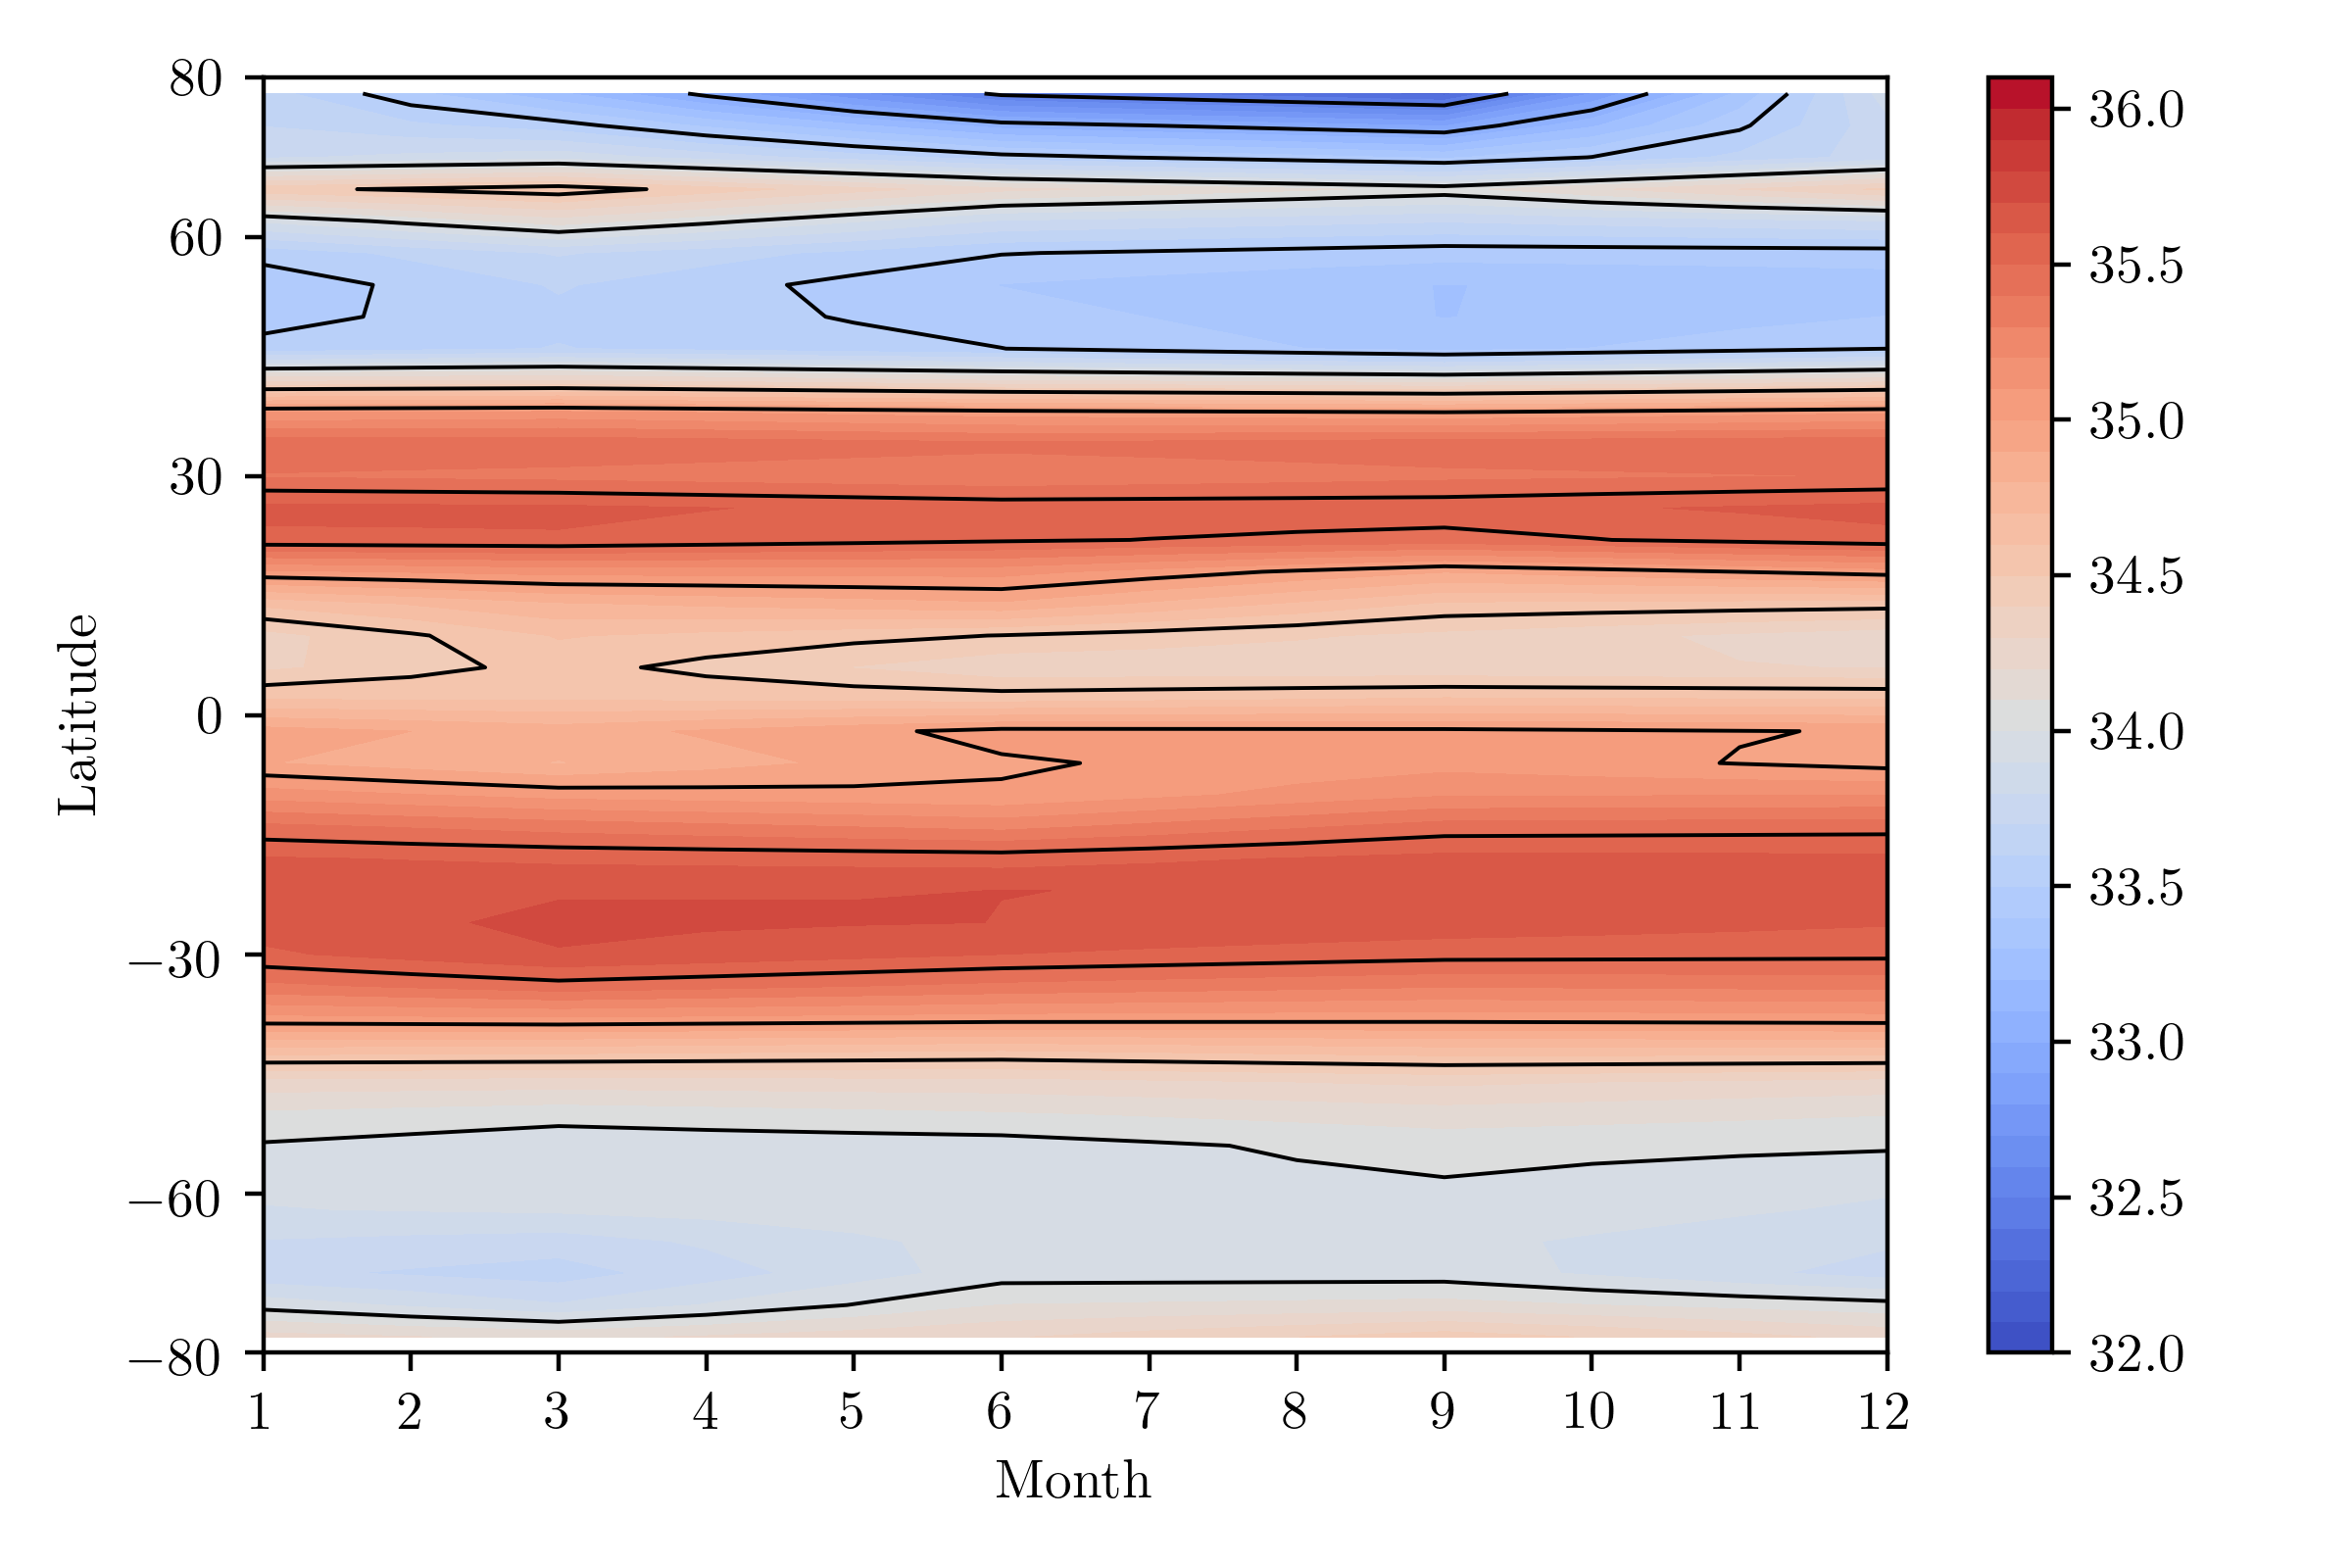
\includegraphics[width=\linewidth]{sss_profile.png}
\end{subfigure}
\begin{subfigure}{.5\textwidth}
	\caption{$\tau_x$ profile ($Nm^{-2}$)}
	\label{fig:tau_profile}
	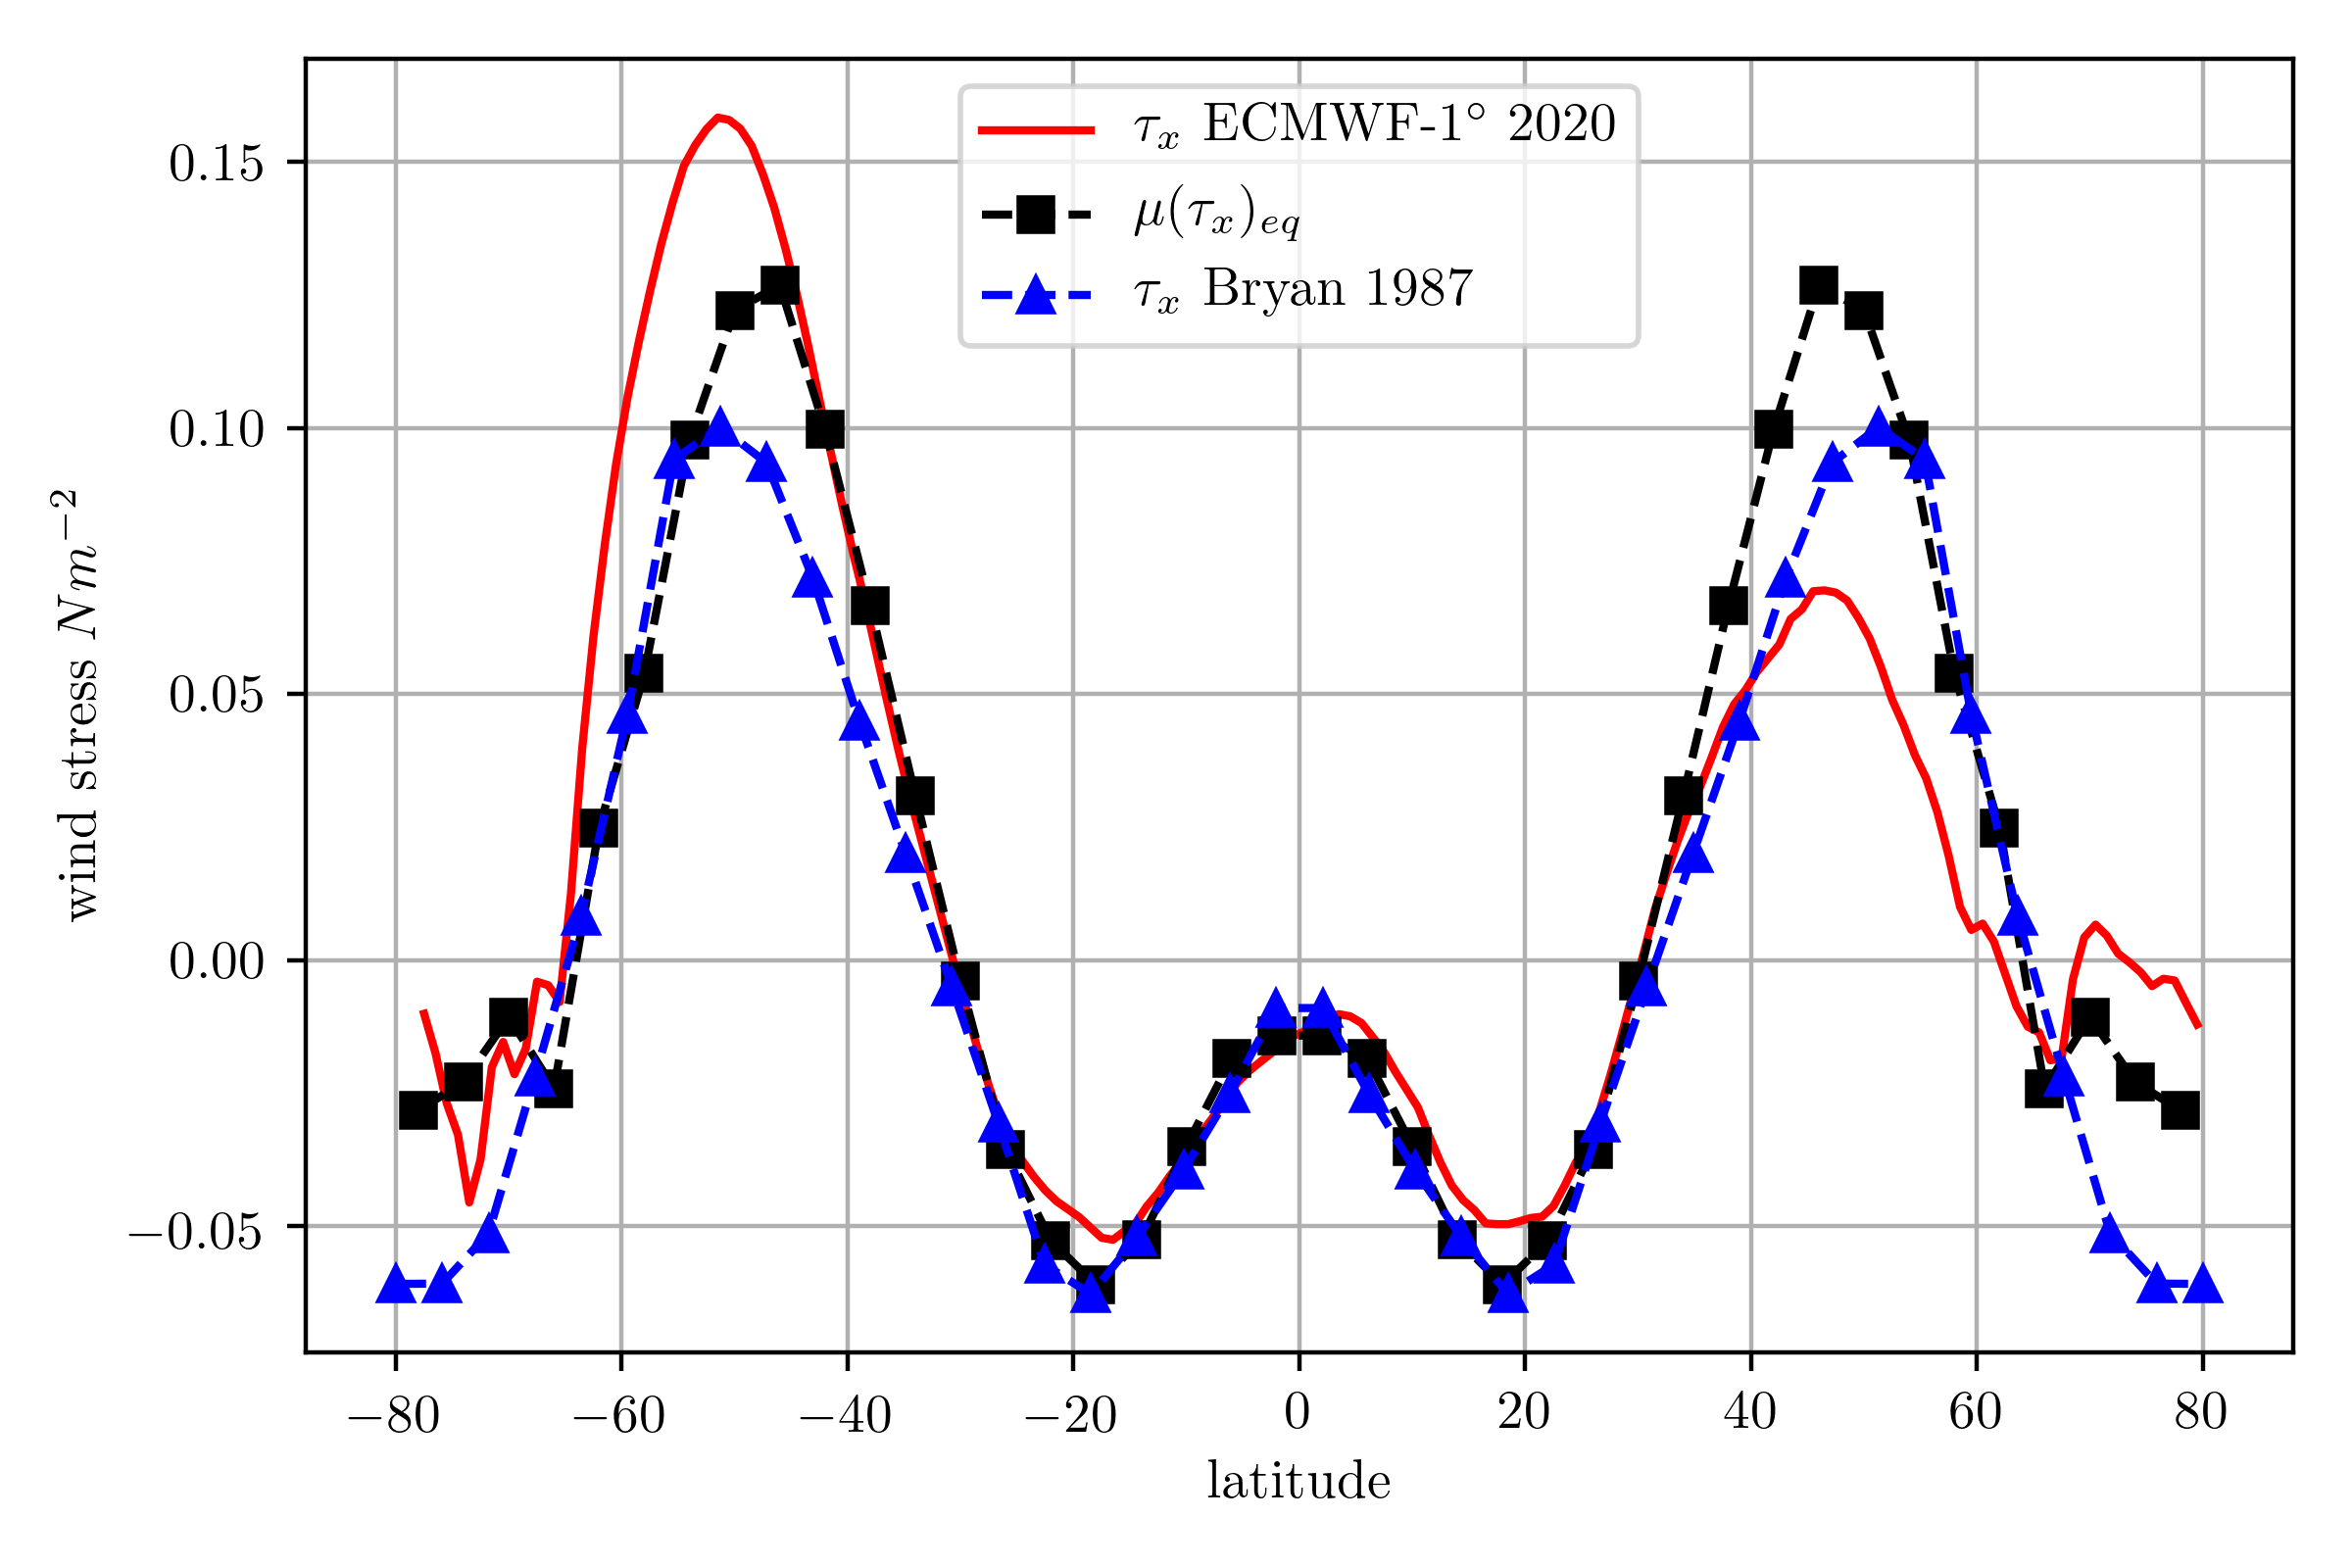
\includegraphics[width=\linewidth]{windstress_models.png}
\end{subfigure}
\caption{Zonal mean annual forcing profiles for \textbf{a)} The net monthly surface heat flux forcing profile for each latitude. Showing large annual variation in surface heat flux. \textbf{b)} The monthly Sea Surface Temperature (SST) forcing profile. Showing annual variation in the net surface temperature. \textbf{c)} Sea Surface Salinity (SSS) forcing profile showing little annual variation. \textbf{d)} The zonal wind stress profiles ($\tau_x$) that were looked at. The red line shows the zonal average of the $ECMWF-1^{\circ}$ forcings. The black squares show zonally averaged $ECMWF-4^{\circ}$ forcings that were mirrored along the equator. The Blue triangles show analytic forcing profile from \cite{bryan1987parameter}}
\label{fig:idealized_forc}
\end{figure}
\newpage
\begin{multicols}{2}
 \subsubsection{Forcing bias} \label{sec:forc_err}
The forcings used in this paper have large errors compared to the present day realistic forcings. This can be seen if we compare them to their original realistic forcings. In \cref{fig:sss_sst_errors} the errors compared to present-day forcings are shown. There is a large discrepancy in the Atlantic, which has a much higher salinity in the realistic forcings than in the idealized forcings. This may have implications on the thermohaline circulation we will observe in our model. It is furthermore noted that the northern Atlantic ocean is much warmer in reality than in our model, which again possibly can affect the thermohaline circulation.
Furthermore, it is also noted that the temperature on earth was also much higher in the early part of the 65Ma period (\cite{Hansen2013Oct}). We neglect this effect because we use the same forcing for each time step. Therefore, it is not possible to compare our results directly with existing proxies. However, studying the effect of geometry changes specifically is much clearer using this method and allows a deeper insight in changes induced by the geometry.
 \subsubsection{Initial conditions}
The model is started with an initial temperature and salinity profile. The profile is scaled from forcings taken from observational data (\cite{ECMWFForc}). The profiles again use zonal means. This results in the profile seen for the situation around the equator in \cref{fig:salt_temp_prf}.

\begin{figure}[H]
	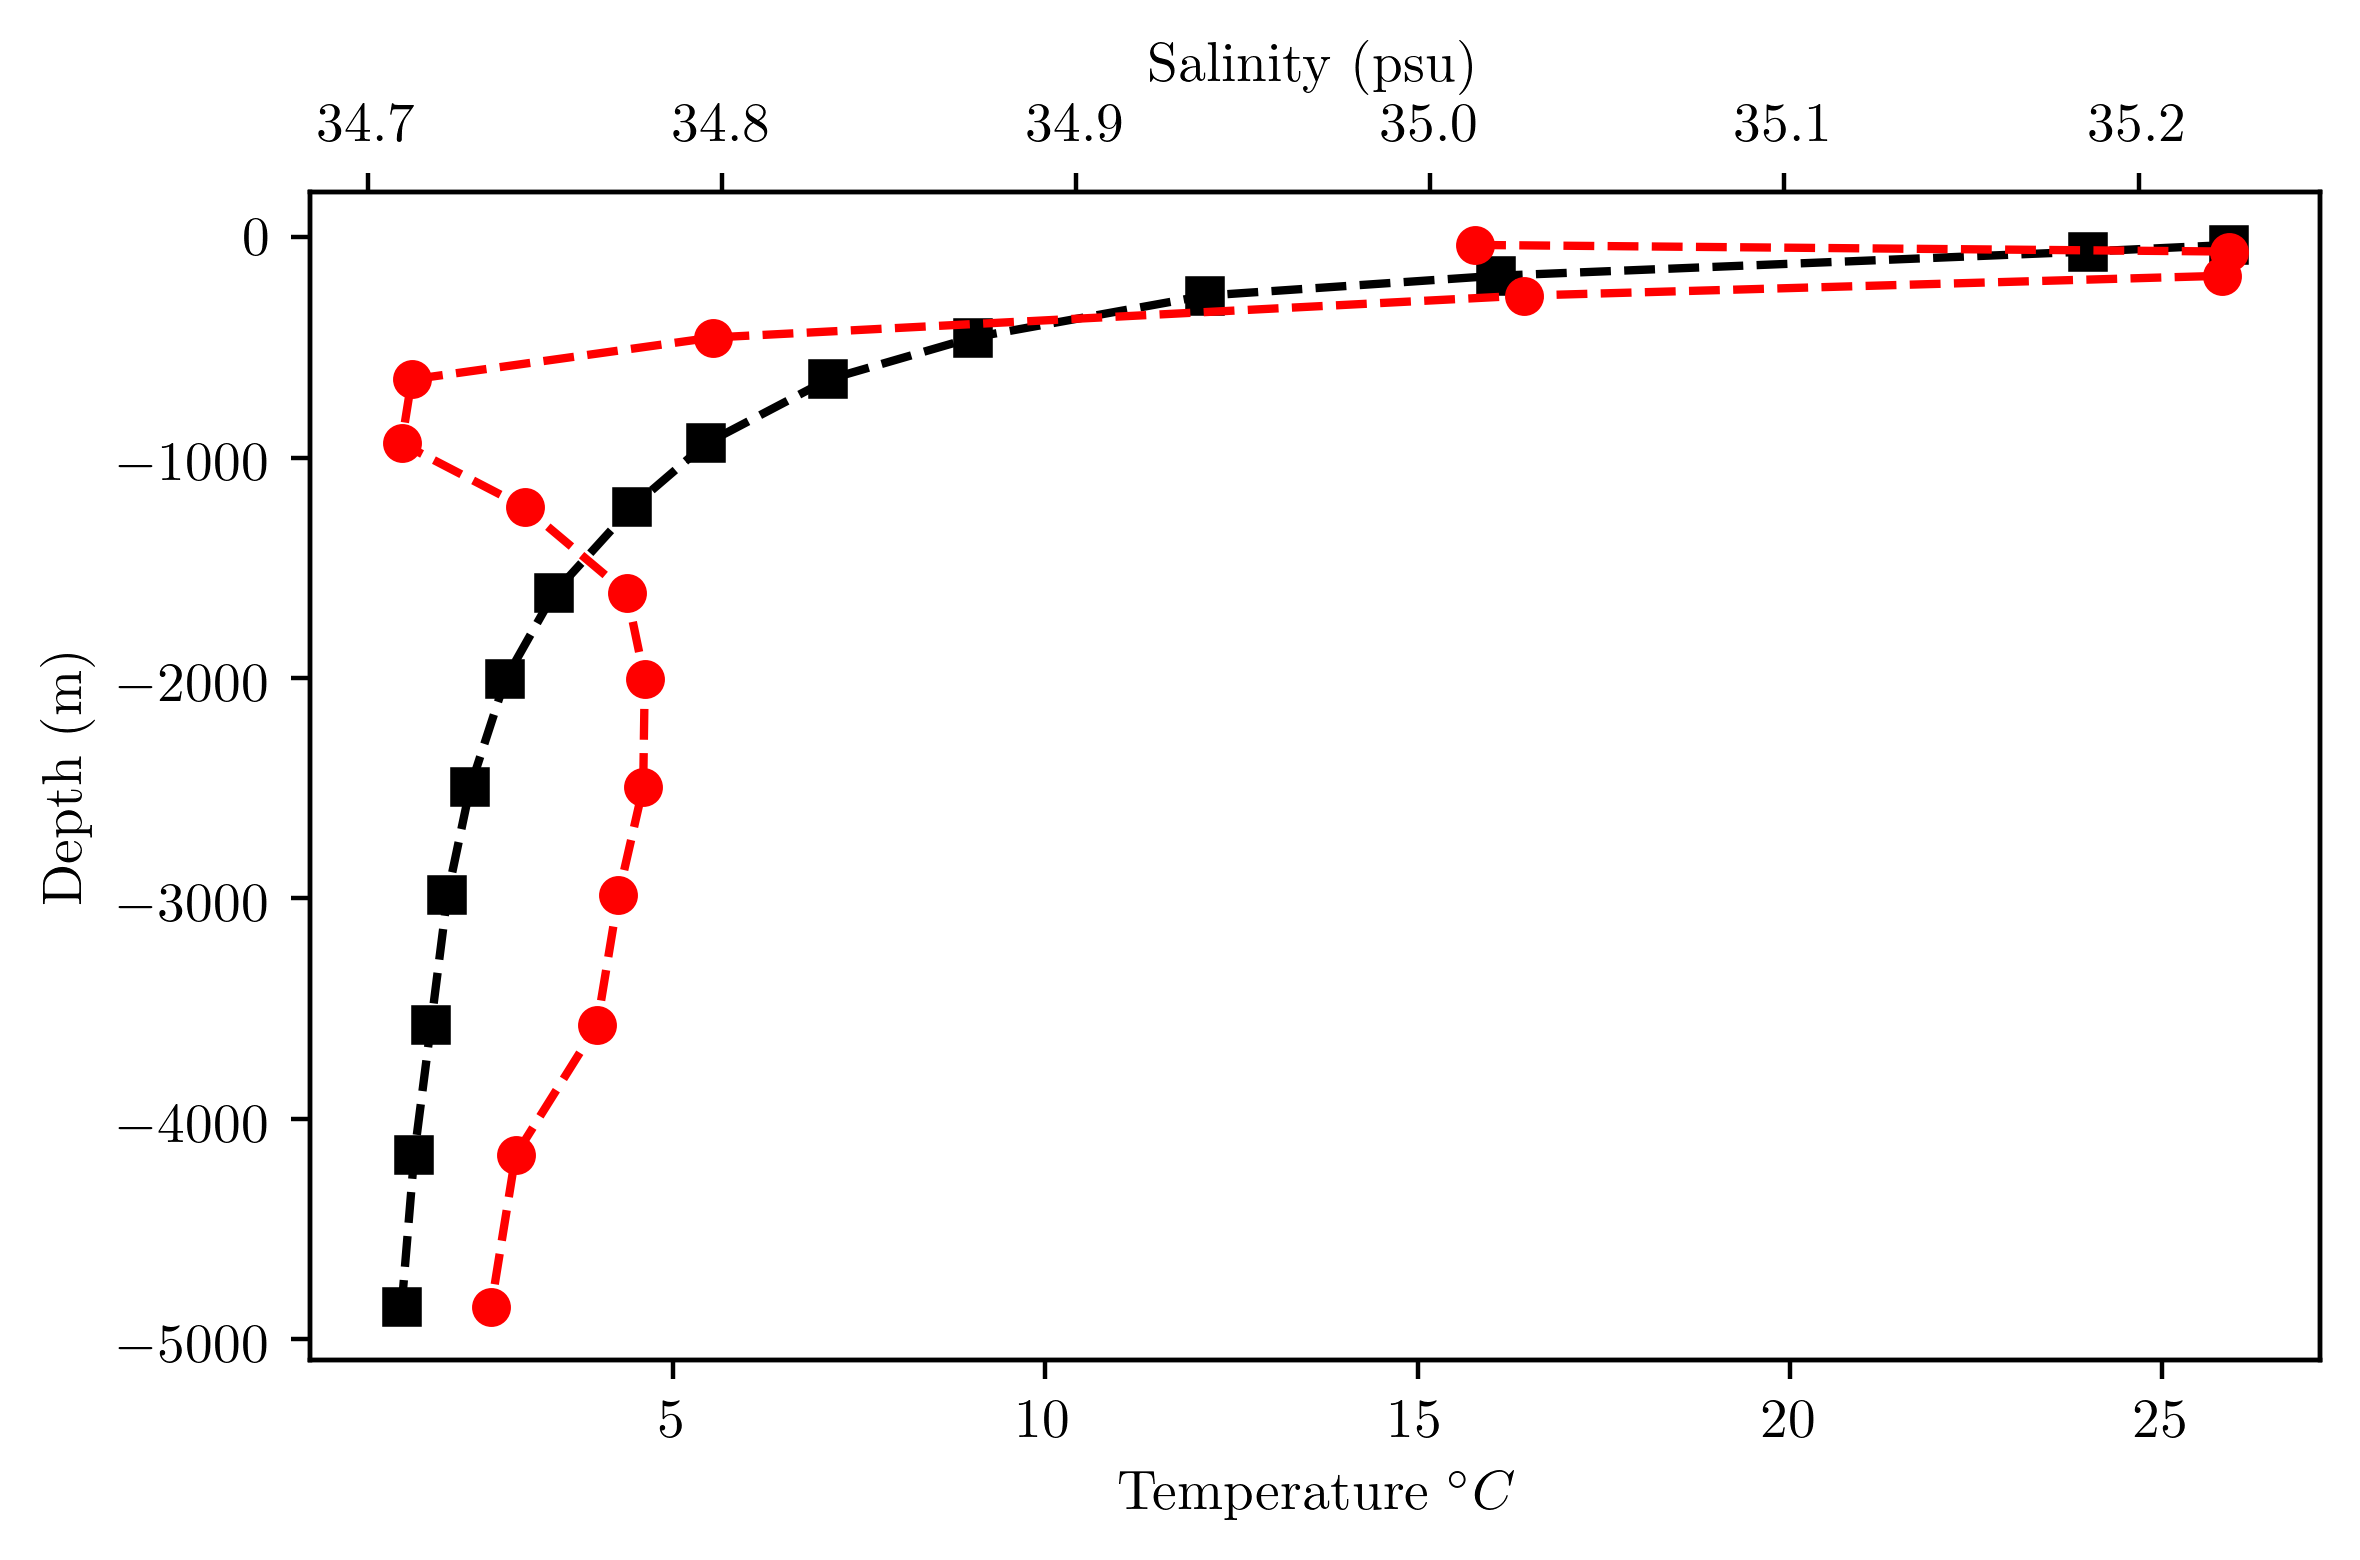
\includegraphics[width=1\linewidth]{salt_temp_prof.png}
	\caption{Temperature and salinity profiles at $2^{\circ} N$. Black squares indicate the Temperature ($^{\circ}C$) profile and red circles indicate the salinity($psu$) profile. Profiles from \cite{ECMWFForc} scaled to 15 depth layers with grid stretching.}
	\label{fig:salt_temp_prf}
\end{figure}
\end{multicols}
\begin{figure}[H]
	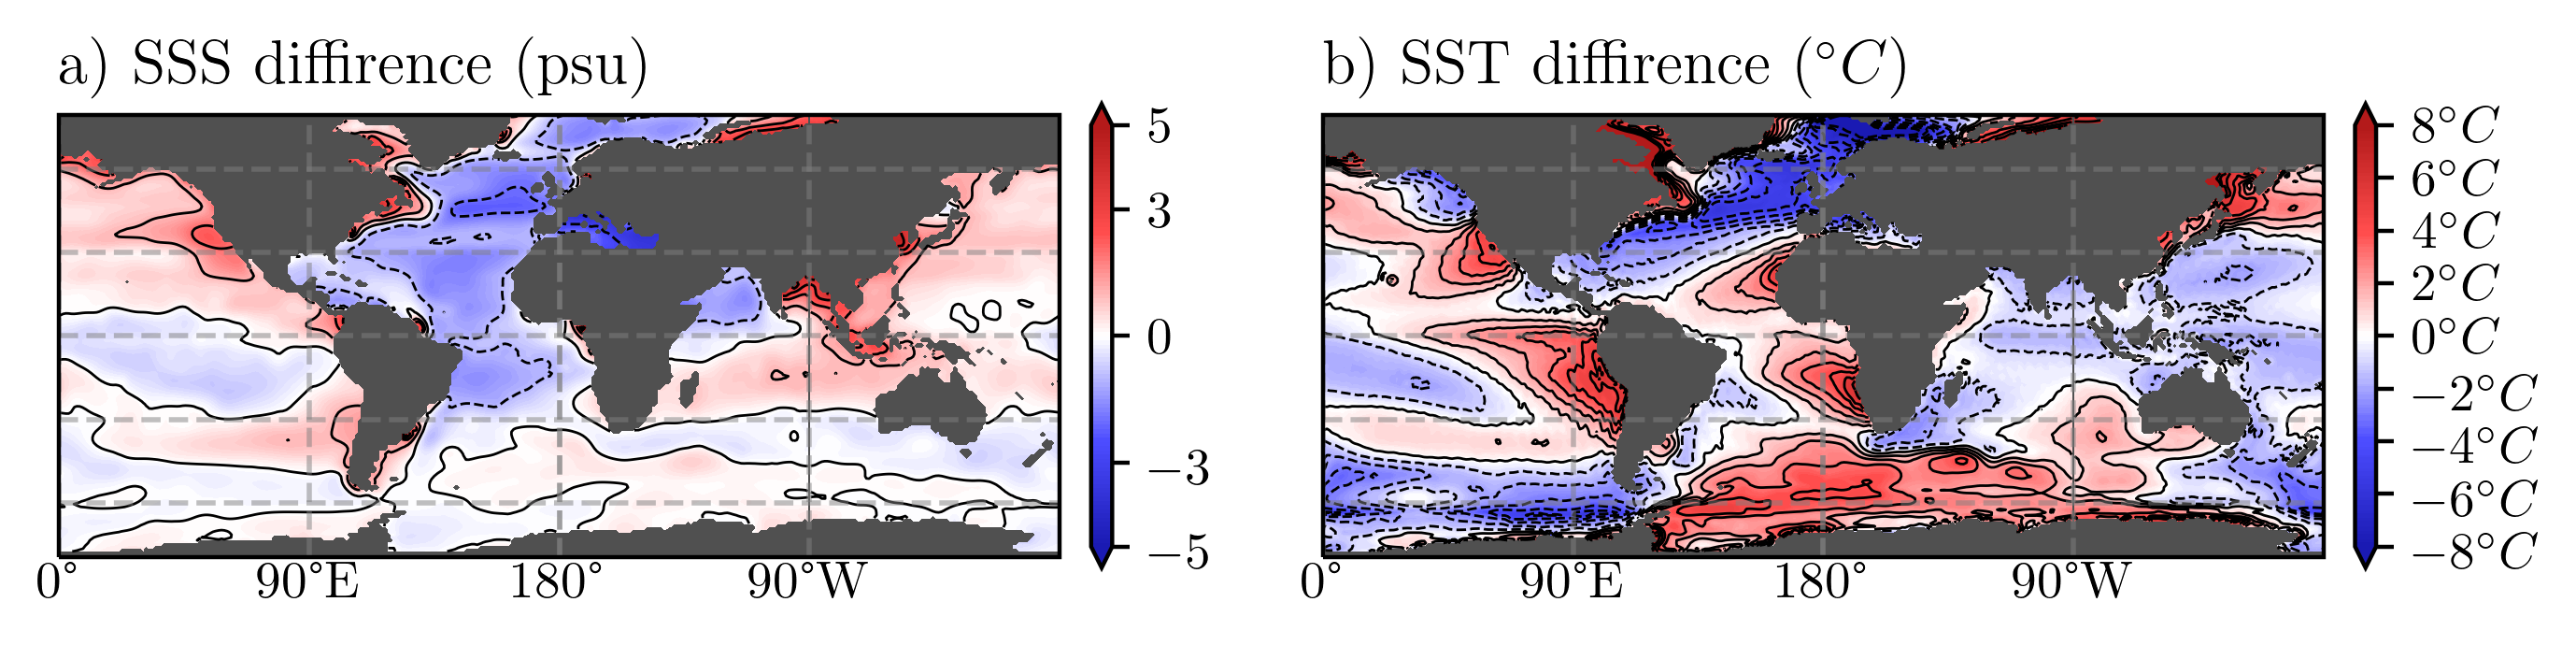
\includegraphics[width=\linewidth]{SST_SSS_errors.png}
	\caption{Errors in surface forcing. As a difference between ECMWF-$1^{\circ}$ forcings and their zonal mean.  Here positive values are over estimations of the forcings. Errors for: \textbf{a)} the SSS difference with contours every 1 psu and \textbf{b)} the SST difference with contours every 1 $^{\circ}C$}
	\label{fig:sss_sst_errors}
\end{figure}
\newpage
\begin{multicols}{2}
\subsubsection{MOC stream function} \label{sec:MOCSTREAM}
The global Meridional Overturning Circulation $\Psi_{MOC}$ is defined as the zonally integrated meridional volume transport of water in the worlds oceans. It can be written down as:
\begin{align}
	\Psi_{MOC}(y,z) = \int_{z}^{0} \int_{180^{\circ}E}^{180^{\circ}W} v(x,y,z') dx dz'.
\end{align}

Here $v$ is the meridional component of the velocity.
$ \Psi_{MOC}$ is thus a stream function of the zonally integrated volume transport in the Earth's ocean basins. Plotting this stream function can give a lot of insight into the deep water transport associated with the thermohaline circulation. In this paper, we hope to capture these deepwater transport formations. In particular, we are looking for the shape of the North Atlantic deep water (NADW) and the Antarctic Bottom Water (AABW) formations (\cref{fig:moc_ex}).

 \begin{figure}[H]
	\includegraphics[width=\linewidth]{moc_example.png}
	\caption{Meridional overturning circulation from observations taken from \cite{Forget2015Oct}. With schematic arrows indicating flow direction. Also including locations of major overturning flows. AABW: Antarctic Bottom Water, NADW: North Atlantic Deep Water, NPIW: North Pacific Intermediate Water,  SAMW: Subantarctic Mode Water, AAIW: Antarctic intermediate Water, ACC Antarctic Cicumpolar Current.}
	\label{fig:moc_ex}
\end{figure}

\subsubsection{Barotropic Stream Function} \label{sec:BSF_theory}
It is furthermore interesting to look at an expression for the transport of ocean gyres. We know that the depth-integrated flow must be horizontally non-divergent. Thus a stream function $\Psi_{b}$ can be introduced:
\begin{align}
U = -\frac{\partial \Psi_{b}}{\partial y}; V=\frac{\partial \Psi_{b}}{\partial x} \label{eq:psiv} \\
\Psi_{b}(x, y) = \int_{eastern bdy}^{x} \int_{-D}^{0} v(x',y,z) dz dx'.
\end{align}
Here $v(x,y,z)$ is the meridional velocity and $u(x,y,z)$ is the zonal flow.
This so-called barotropic stream function (BSF) $\Psi_{b}$ is defined by integrating the meridional transport westward from the eastern boundary of the domain. It is a useful tool to look at the shape and gyres associated with the major ocean current systems. By using the Sverdrup relation:
\begin{align}
	\int_{-D}^{0}v(x,y,z) dz = \frac{1}{\beta \rho_{ref}}\vec{\hat{z}}\cdot \nabla \times \tau
\end{align}

which was first proposed by \cite{sverdrup1947wind}. We can look at a schematic diagram of the barotropic stream function based on the prevailing zonal winds (\cref{fig:schem_currents}). It is clear that the prevailing zonal winds relate to the wind stress forcing seen in \cref{fig:idealized_forc}. The calculation of the barotropic stream function without easily defined boundaries is quite a bit more cumbersome than a simple integration from the eastern boundary. Veros uses a process in which special treatment is given to boundaries using something called island integrals. This is why the barotropic stream function has values below the land mask in Veros. 
 
  \begin{figure}[H]
 	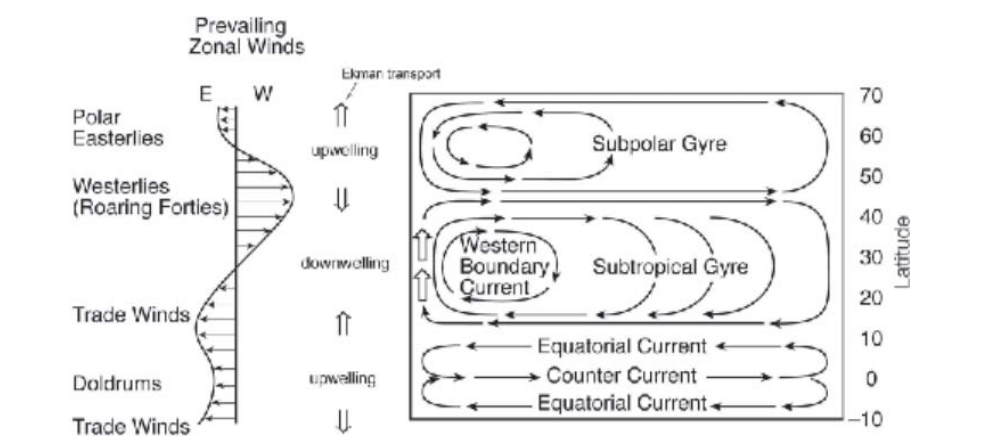
\includegraphics[width=\linewidth]{schematic_marshall_plumb.png}
 	\caption{Schematic of the barotropic stream function based on the Sverdrup relation. Showing the subpolar and subtropical Gyres and equatorial currents. Figure taken from \cite{MarschallPlumb}}
 	\label{fig:schem_currents}
 \end{figure}
\newpage
\subsubsection{Passage throughflow}\label{sec:throughflowp}
For passages between larger oceanic basins it is interesting to look at the total transported volume of water and the direction of this flow. The location of the passages that will be studied can be seen in \cref{fig:passages_ocean}. The volume transport in the zonal direction through an area $A$ is defined as
\begin{align}
Q = \iint_A u(x,y,z) dA. \label{eq:tranpss}
\end{align}	
Here, we integrate the zonal velocity over an area $A$ in the latitude-vertical direction that is normal to this velocity. By applying \cref{eq:psiv} to \cref{eq:tranpss} we can use the output of the BSF $\Psi_b$ to find the zonal volumetric flux through each grid cell in our model. We use the BSF output over the velocity output because the BSF is more accurate than the velocity field. This is because the velocity field is a derived quantity in Veros, while the BSF is calculated every integration step.

For each passage a suitable location is chosen such that there are no boundaries next to the passageways, this is done for each time step. In \cref{fig:passages_def} an example of this method is shown for 20Ma. This method is the same for each of the passages and thus we can study the effect of changes in bathymetry on the relative strength of the flow. However, it should be noted that these values may not represent real physical values. In \cref{fig:passages_ocean} An overview is shown of all the passages discussed in this paper.


\begin{figure}[H]
	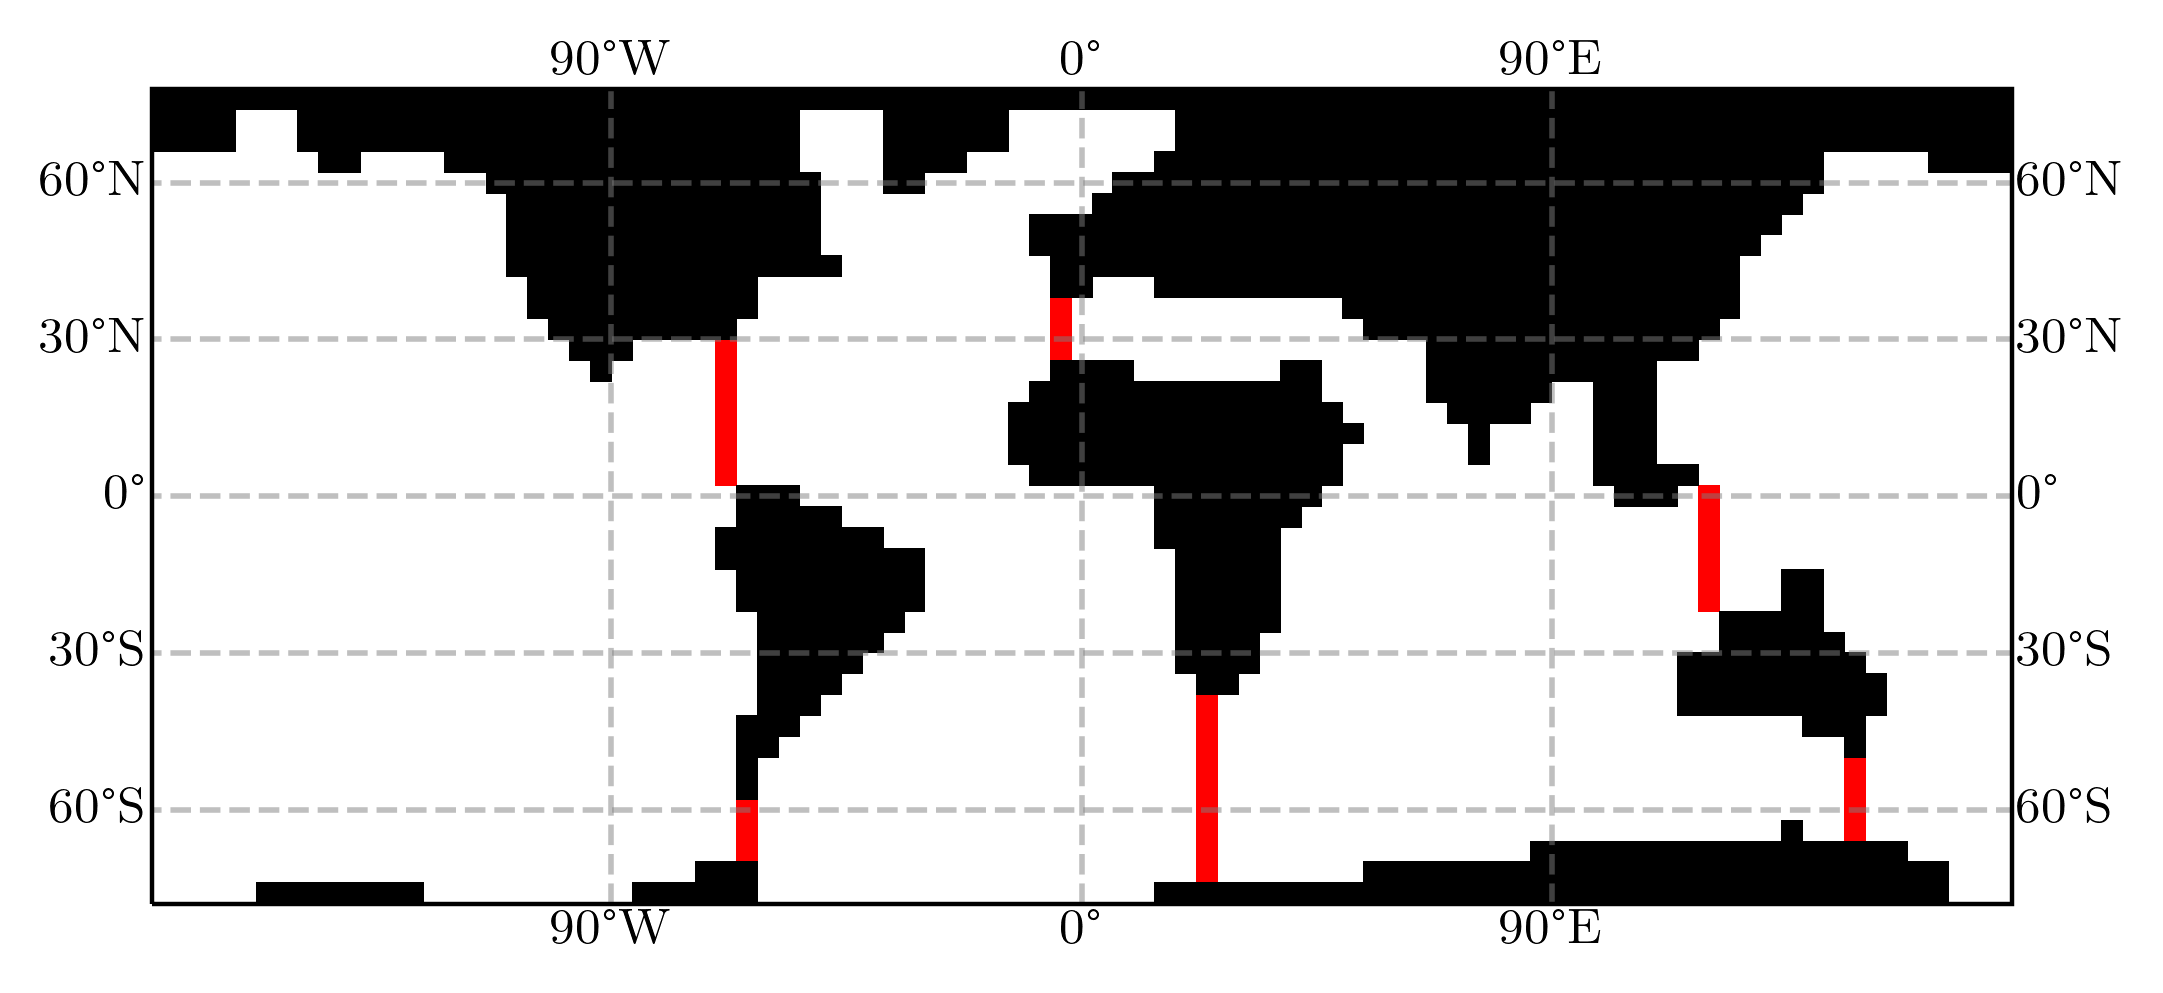
\includegraphics[width=\linewidth]{def_pass.png}
	\caption{Example of the chosen grid cells for individual passages for 20Ma. The land mask shown here is the land mask excluding grid cells used for the BSF boundary conditions and is thus not the same as the land mask used for the model itself.}
	\label{fig:passages_def}
\end{figure}

\end{multicols}
 \begin{figure}[H]
	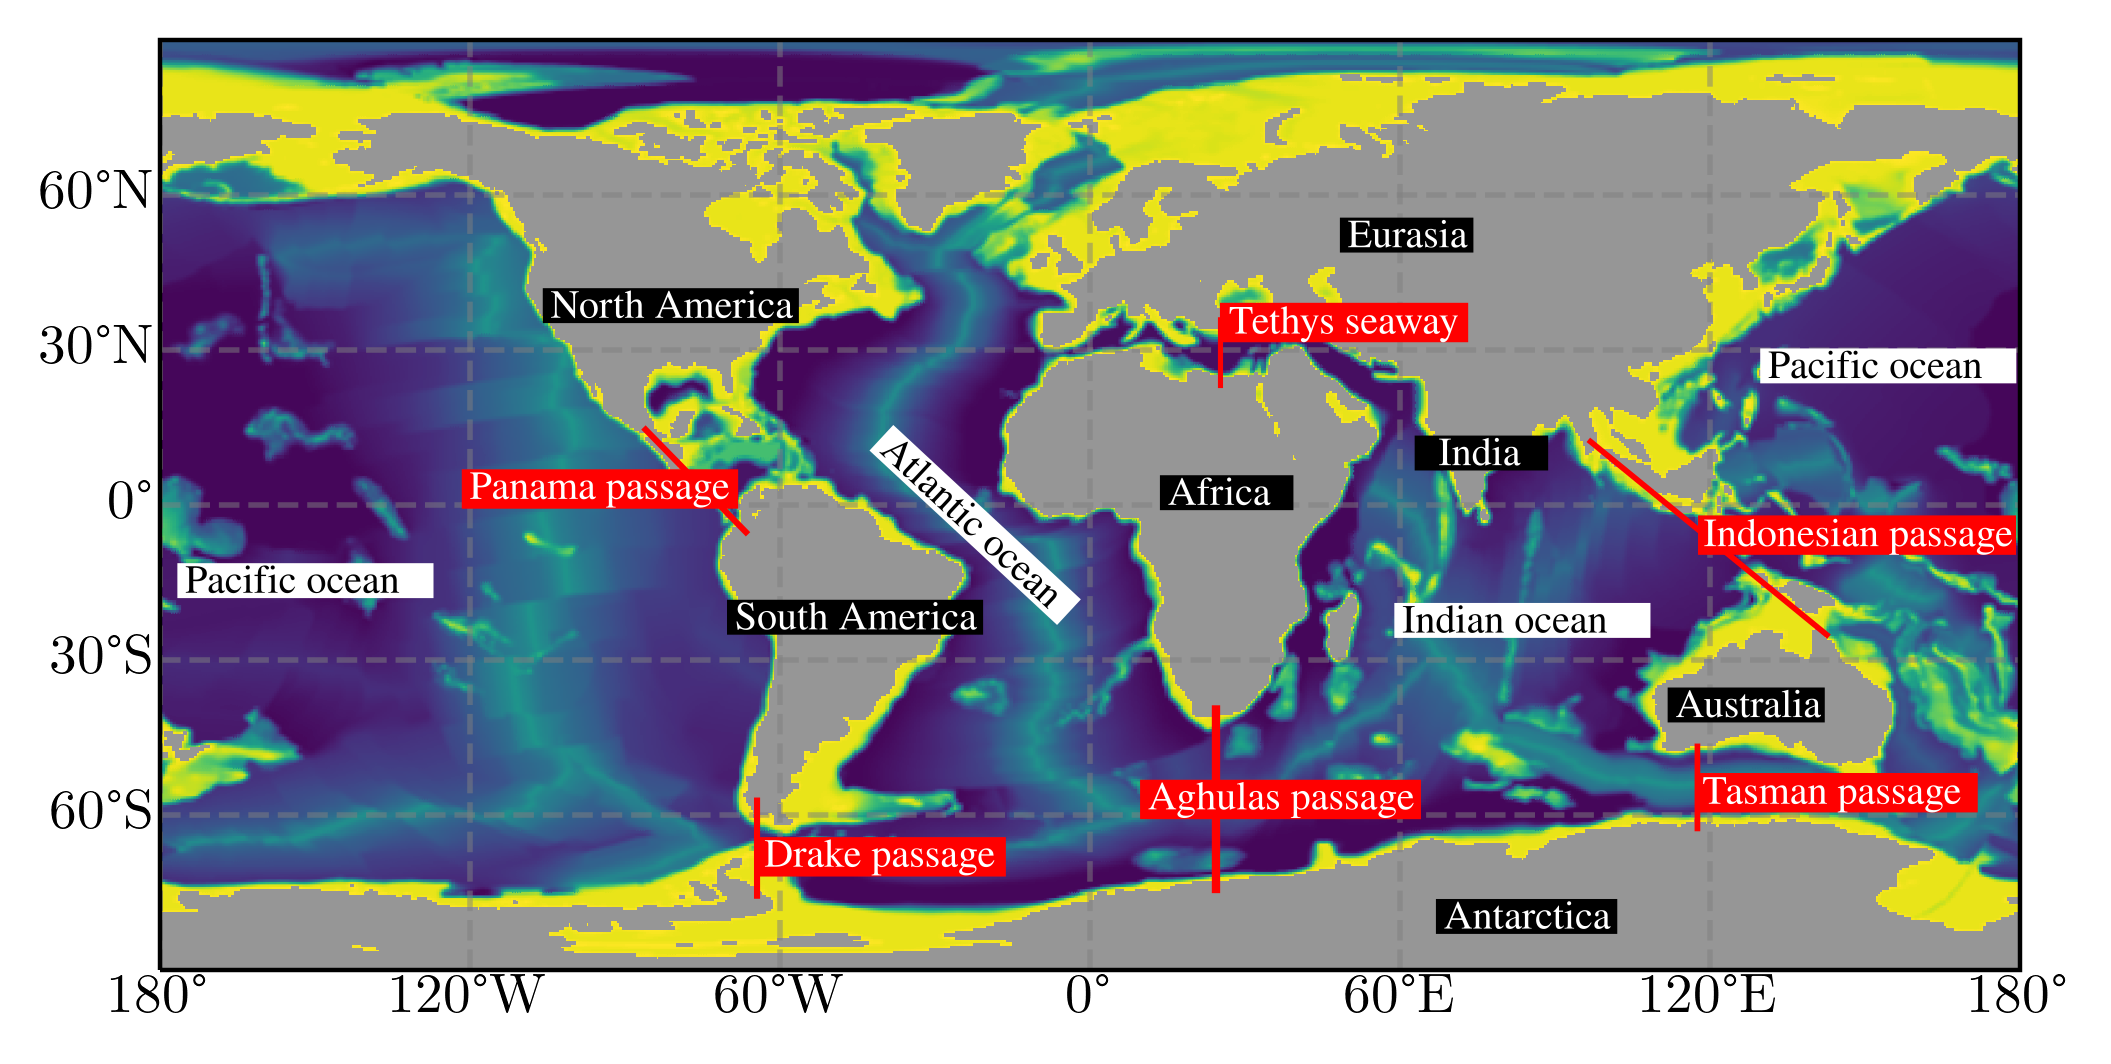
\includegraphics[width=\linewidth]{passages_oceans.png}
	\caption{Schematic image showing the 30 Ma bathymetry in $0.5^{\circ} \times 0.5^{\circ} $. Overlayed in red are the passages we study. In black the continents and in white the oceanic basins.}
	\label{fig:passages_ocean}
\end{figure}
\begin{multicols}{2}